With EMF Refactor and Henshin conditions can be designed either as
'initialCheck', 'finalcheck' or as 'execute'.
\\\\
Where initial- and finalcheck serve as preconditional check, the 'execute'-type
is the actual transformation which does the modification.

Note, with finalchecks one designes the 'negative' case which is not wanted for
the execution to be run - or in other words: the finalcheck must NOT match for
the 'execute' to be run.

%----------Pre:checkOtherNames----------------------------------------
\cond
{Precondition: checkOtherNames}
{checkOtherNames}
{This precondition is a 'finalcheck'. checkOtherNames
will match if an element (here: UMLClass) with the same name like
in the propagated value of 'newName' exists under the selected context (here:
UMLPackage) and therefore prevent the actual transformation process.
\\\\
In other words: the finalcheck mustn't match if one wants the corresponding
'execute' (here e.g. createClass or editClassName) to be run.}

\begin{figure}[H]
  \centering
  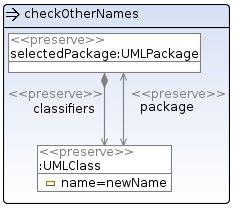
\includegraphics[width=0.4\textwidth]{pics/cond_checkOtherNames.png}
  \caption{checkOtherNames}
  \label{checkOtherNames}
\end{figure}
%----------Pre:checkOppositeAggregationKind---------------------------
\cond
{Precondition: checkOppositeAggregationKind}
{checkOppositeAggregationKind}
{still to be implemented}
%----------Pre:checkInheritanceCycle----------------------------------
\cond
{Precondition: checkInheritanceCycle}
{checkInheritanceCycle}
{still to be implemented}
